\documentclass{article}
\usepackage[utf8]{inputenc}

\title{MLT Homework 4}
%\author{Ana Borovac \\ Jonas Haslbeck \\ Bas Haver} % I'll be coming back :-)
\author{Ana Borovac  \\ Bas Haver}

\usepackage{natbib}
\usepackage{graphicx}
\usepackage{subcaption}

\usepackage{amsmath}
\usepackage{amsfonts}
\usepackage{amssymb}
\usepackage{bbm}
\usepackage{mathtools}

\usepackage{url}

\DeclarePairedDelimiter\ceil{\lceil}{\rceil}
\DeclarePairedDelimiter\floor{\lfloor}{\rfloor}

\newcounter{counterquestion}
\newenvironment{question}[1]
{
\stepcounter{counterquestion}
\section*{Question \thecounterquestion}
\emph{#1} 
} 
{
}

\newcounter{countersubquestion}[counterquestion]
\newenvironment{subquestion}[1]
{
\stepcounter{countersubquestion}
\subsection*{Subquestion \thecounterquestion .\thecountersubquestion}
\emph{#1} 
} 
{
}

\newenvironment{solution}
{
\subsubsection*{Solution}
} 
{
}


\begin{document}

\maketitle

% 1st question
\begin{question}{We have shown that for a finite hypothesis class $\mathcal{H}$, $\text{VCdim}(\mathcal{H}) \leq \floor*{\log(|\mathcal{H}|)}$. However, this is just an upper bound. The VC-dimension of a class can be much lower than that.}
\begin{subquestion}{Find an example of a class $\mathcal{H}$ of functions over the real interval $\mathcal{X} = [0, 1]$ such that $\mathcal{H}$ is infinite while $\text{VCdim}(\mathcal{H}) = 1$.}
\begin{solution}
Let's define hypothesis class as:
\[
\mathcal{H} = \{h_{a}:\ a \in [0, 1]\}
\]
\[
h_{a}(x) = 
\begin{cases}
1; & x \geq a \\
0; & x < a \\
\end{cases} 
\]
%
From definition we know $|\mathcal{H}| = \infty$. Now we need to prove that $\text{VCdim}(\mathcal{H}) = 1$.

\begin{figure}[h!]
    \centering
    \begin{subfigure}[t]{0.4\textwidth}
        \centering
        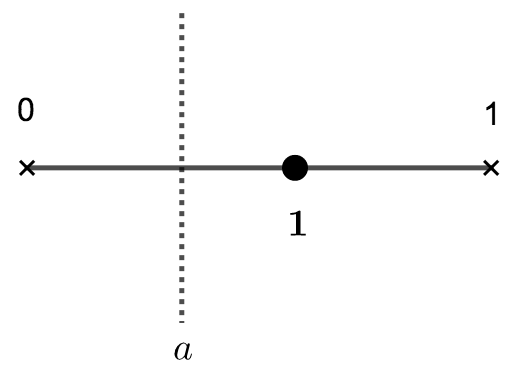
\includegraphics[width=0.9\textwidth]{Question11.png}
        \caption{If point is labeled “1”.}
    \end{subfigure}
    \begin{subfigure}[t]{0.4\textwidth}
        \centering
        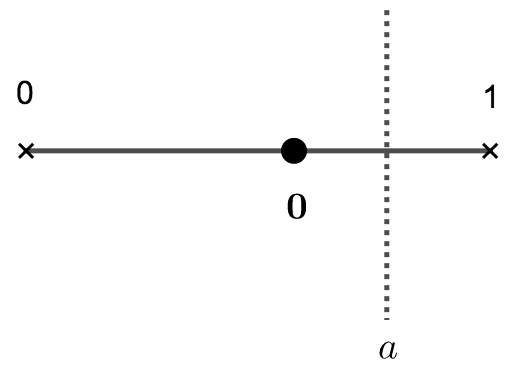
\includegraphics[width=0.9\textwidth]{Question12.png}
        \caption{If point is labeled “0”.}
    \end{subfigure}
    \caption{Proof that $\text{VCdim}(\mathcal{H}) \geq 1$.}
    \label{fig: question111}
\end{figure}

\begin{itemize}
\item $\text{VCdim}(\mathcal{H}) \geq 1$: The proof we can see from the figure \ref{fig: question111}.
\item $\text{VCdim}(\mathcal{H}) \leq 1$: From the figure \ref{fig: question112} it is seen that hypothesis class $\mathcal{H}$ does not shatter a set of two points (no matter how we position them).
\end{itemize}

\begin{figure}[h!]
\centering
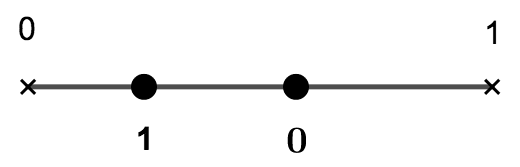
\includegraphics[width=0.5\textwidth]{Question13.png}
\caption{The problem we have when trying to shatter a set of two points.}
\label{fig: question112}
\end{figure}
\end{solution}
\end{subquestion}

\begin{subquestion}{Give an example of a finite hypothesis class $\mathcal{H}$ over domain $\mathcal{X} = [0, 1]$, where $\text{VCdim}(\mathcal{H}) = \floor*{\log_2(|\mathcal{H}|)}$}
\begin{solution}
Let's define hypothesis class:
\[
\mathcal{H} = \{h_0, h_1\}
\]
where $h_0(x) = 0$ ($\forall x$) and $h_1(x) = 1$ ($\forall x$). We would like to prove that $\text{VCdim}(\mathcal{H}) =  \floor*{\log_2(|\mathcal{H}|)} =  \floor*{\log_2(2)} = 1$.
\begin{itemize}
\item $\text{VCdim}(\mathcal{H}) \geq 1$: If we want to label a $x \in [0, 1]$ as 1, we pick $h_1$ as hypothesis, otherwise we pick $h_0$. So, $\text{VCdim}(\mathcal{H}) \geq 1$.
\item $\text{VCdim}(\mathcal{H}) \leq 1$: Let say that we have a set of two points. If we want to label one of the point with 1 and the other with 0, there does not exist a hypothesis in hypothesis class which can label two points differently. 
\end{itemize}
We can conclude that $\text{VCdim}(\mathcal{H}) = 1$.
\end{solution}
\end{subquestion}
\end{question}


% 2nd question
\begin{question}{It is often the case that the VC-dimension of a hypothesis class equals (or can be bounded above by) the number of parameters one needs to set in order to define each hypothesis in the class. For instance, if $\mathcal{H}$ is the class of axis aligned rectangles in $\mathbb{R}^d$, then VCdim$(\mathcal{H})=2d$, which is equal to the number of parameters used to define a rectangle in $\mathbb{R}^d$. Here is an example that shows that this is not always the case. We will see that a hypothesis class might be very complex and even not learneble, although it has a small number of parameters.\\
Consider the domain $\mathcal{X}=\mathbb{R}$, and the hypothesis class $$\mathcal{H}= \{ x\mapsto \ceil{\sin (\theta x) }:\theta \in \mathbb{R} \}$$
(here, we take $\ceil{-1}=0$). Prove that VCdim$(\mathcal{H})=\infty$.\\
\textit{Hint:} There is more than one way to prove the required result. One option is by applying the following lemma: If $-.x_1x_2x_3\dots ,$ is the binary expansion of $x\in (0,1)$, then for any natural number $m$, $\ceil{\sin (2^m \pi x)}=(1-x_m)$, provided thath $\exists k \geq m$ s.t. $x_k=1$.}
\begin{solution}
Assume VCdim$(\mathcal{H})=k<\infty$. We will reach towards a contradiction by finding $k+1$ elements which are shattered by $\mathcal{H}$, from which we can conclude that VCdim$(\mathcal{H})=\infty$. All these $k+1$ elements will be found in the interval $(0,1)$, such that they can be written as a binary expansion. We choose our elements to have all different combinations of zeros and ones for every entry of the $x_m$. This can of course be done in multiple way, we just choose one. For example $x_1$ can be chosen to be one for all elements, $x_2$ one for all elements except for the first element, where we choose $x_2$ to be zero, $x_3$ one for all elements except for the second one, where we choose $x_3$ zero. We proceed this way until we have $x_{2^{k+1}}$ all zero. Now place a one for $x_{2^{k+1}+1}$ in order to always be able to apply the lemma as stated in the hint. Note now that all these elements are different, so that we really have contructed $k+1$ elements. Now the lemma as in the hint gives us, when we choose $\theta=2^m\pi$, that we label $\ceil{\sin (\theta x)}=1-x_m$. So if $x_m=1$ we label it zero and if $x_m=0$ we label it one. Now for any combination of the $k+1$ elements we can fix an arbitrarily chosen labeling. This labeling can then be constructed by choosing $m$ such that $x_m$ would give the 'opposite' labeling (which is such that $1-x_m$ is the admired labeling). This $m$ exists by construction. Since our labeling was fixed arbitrarily, we can construct any labeling. Therefore our $k+1$ elements are shattered by $\mathcal{H}$.\\
Since we assumed VCdim$(\mathcal{H})=k<\infty$ and found $k+1$ shattered elements, we have a contradiction and conclude VCdim$(\mathcal{H})=\infty$.
\end{solution}
\end{question}


% 3rd question
\begin{question}{Let $\mathcal{H}$ be the class of signed intervals, that is, $\mathcal{H} = \{h_{a, b, s} : a \leq b, s \in \{-1, 1\}\}$ where
\[
h_{a, b, s}(x) =
\begin{cases}
s & \text{if}\ x \in [a, b] \\
-s & \text{if}\ x \notin [a, b] 
\end{cases}
\]
Calculate $\text{VCdim}(\mathcal{H})$.}
\begin{solution}
Claim: $\text{VCdim}(\mathcal{H}) = 3$.

\begin{itemize}
\item $\text{VCdim}(\mathcal{H}) \geq 3$: On figure \ref{fig: question31} it is seen that set of three points can be shattered. Furthermore $\text{VCdim}(\mathcal{H}) \geq 3$.

\begin{figure}[h!]
    \centering
    \begin{subfigure}[t]{0.4\textwidth}
        \centering
        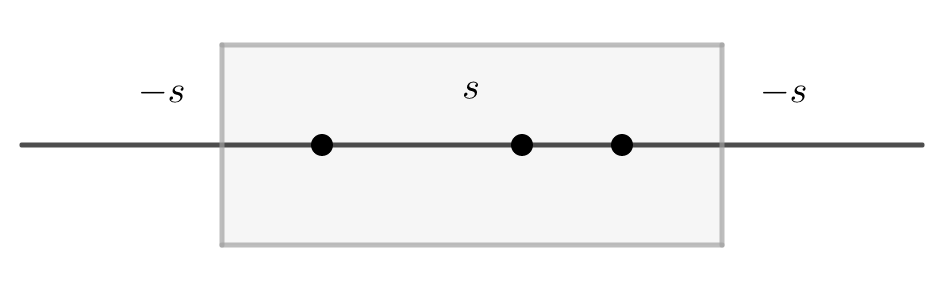
\includegraphics[width=0.9\textwidth]{Question31.png}
        \caption{}
    \end{subfigure}
    \begin{subfigure}[t]{0.4\textwidth}
        \centering
        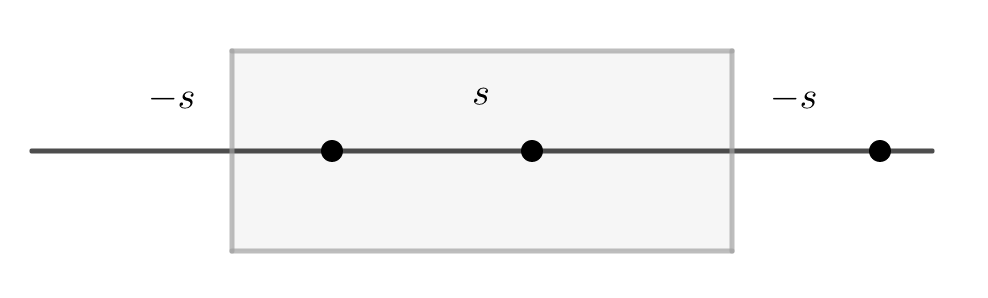
\includegraphics[width=0.9\textwidth]{Question32.png}
        \caption{}
    \end{subfigure}
     \begin{subfigure}[t]{0.4\textwidth}
        \centering
        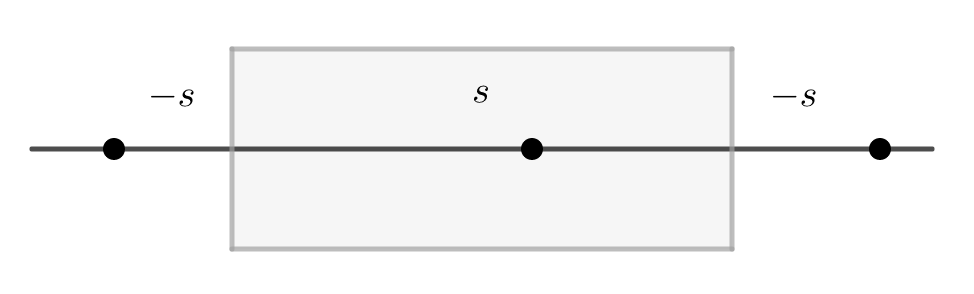
\includegraphics[width=0.9\textwidth]{Question33.png}
        \caption{}
    \end{subfigure}
     \begin{subfigure}[t]{0.4\textwidth}
        \centering
        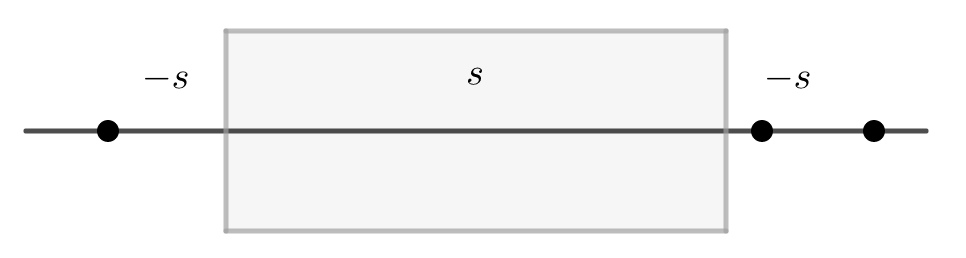
\includegraphics[width=0.9\textwidth]{Question34.png}
        \caption{}
    \end{subfigure}
    \caption{Proof that $\text{VCdim}(\mathcal{H}) \geq 3$.}
    \label{fig: question31}
\end{figure}

\item $\text{VCdim}(\mathcal{H}) \leq 3$: There does not exist a hypothesis $h \in \mathcal{H}$ that lables the situation on figure \ref{fig: question32}. From here we can conclude $\text{VCdim}(\mathcal{H}) \leq 3$.

\begin{figure}[h!]
    \centering
        
\includegraphics[width=0.9\textwidth]{Question35.png}
    \caption{Proof that $\text{VCdim}(\mathcal{H}) \leq 3$.}
    \label{fig: question32}
\end{figure}

\end{itemize}

\end{solution}
\end{question}


% 4th question
\begin{question}{\textbf{VC of union:} Let $\mathcal{H}_1,\dots, \mathcal{H}_r$ be hypothesis classes over some fixed domain set $\mathcal{X}$. Let $d = \max_i \text{VCdim}(\mathcal{H}_i)$ and assume for simplicity that $d \geq 3$.}
\begin{subquestion}{Prove that
\[
\text{VCdim}(\cup_{i = 1}^r \mathcal{H}_i) \leq 4d \log_2 \left(\frac{2d}{\ln 2}\right) + 2 \log_2 (r).
\]
}
\begin{solution}
First, denote a union class as $\mathcal{H}_{\cup} = \cup_{i = 1}^r \mathcal{H}_i$.
Second, assume that $\text{VCdim}(\mathcal{H}_{\cup}) = k$ and therefore $\mathcal{H}_{\cup}$ shatters a set of $k$ elements . Furthermore, the union class can produce all $2^k$ possible labelings on these elements. 

Let's recall Sauer's lemma: Let $\mathcal{H}$ be a hypothesis class with $\text{VCdim}(\mathcal{H}) \leq d < \infty$. Then for all $m$,
\[
\Pi_{\mathcal{H}}(m) \leq m^d
\]
From our assumption it follows:
\[
\Pi_{\mathcal{H}_{\cup}}(k) = 2^k
\]
The definition of shatter function gives as the following inequality:
\[
\Pi_{\mathcal{H}_{\cup}}(k) \leq \Pi_{\mathcal{H}_{1}}(k) + \cdots + \Pi_{\mathcal{H}_{r}}(k)
\]
Now, we can use Sauer's lemma on each summand:
\[
2^k = \Pi_{\mathcal{H}_{\cup}}(k) \leq \Pi_{\mathcal{H}_{1}}(k) + \cdots + \Pi_{\mathcal{H}_{r}}(k) \leq \underbrace{k^d + \cdots k^d}_r = rk^d
\]
If we use $\log_2$ on the inequality, we get:
\begin{equation}
k \leq d\log_2 k + \log_2 r
\label{eq: quation41}
\end{equation}

In the next step we are going to use Lemma A.2 from the book, which says: Let $a \geq 1$ and $b > 0$. Then $x \geq 4a \log_2\left(\frac{2a}{\ln 2}\right) + 2b \implies x \geq a \log_2(x) + b$.

Let's assume that $\text{VCdim}(\mathcal{H}_{\cup}) > 4d \log_2 \left(\frac{2d}{\ln 2}\right) + 2 \log_2 (r)$. From our first assumption we get:
\[
k > 4d \log_2 \left(\frac{2d}{\ln 2}\right) + 2 \log_2 (r)
\]
Now, we can use Lemma A.2 (where $a = d \geq 3$, $b = \log_2 r > 0$):
\[
k > d\log_2 k + \log_2 r
\]
We got into a contradiction with \eqref{eq: quation41}, this means that our assumption was not correct and it holds:
\[
\text{VCdim}(\mathcal{H}_{\cup}) \leq 4d \log_2 \left(\frac{2d}{\ln 2}\right) + 2 \log_2 (r)
\]
\end{solution}
\end{subquestion}

\begin{subquestion}{Prove that for $r = 2$ it holds that
\[
\text{VCdim}(\mathcal{H}_1 \cup \mathcal{H}_2) \leq 2d + 1
\]
}
\begin{solution}
% https://cs.nyu.edu/~mohri/ml/ml10/sol2.pdf
This question was solved with the help of \cite{question42}.

As same as before:
\[
\Pi_{\mathcal{H}_1 \cup \mathcal{H}_2}(m) \leq \Pi_{\mathcal{H}_1}(m) + \Pi_{\mathcal{H}_2}(m)
\]
Now we use Sauer's lemma:
\[
\Pi_{\mathcal{H}_1 \cup \mathcal{H}_2}(m) \leq \Pi_{\mathcal{H}_1}(m) + \Pi_{\mathcal{H}_2}(m) \leq \sum_{i = 0}^d \binom{m}{i} +  \sum_{i = 0}^d \binom{m}{i}
\]
If we use the fect $\binom{m}{i} = \binom{m}{m - i}$, we get:
\begin{align*}
\sum_{i = 0}^d \binom{m}{i} +  \sum_{i = 0}^d \binom{m}{i} & = \sum_{i = 0}^d \binom{m}{i} +  \sum_{i = 0}^d \binom{m}{m - i} \\
& = \sum_{i = 0}^d \binom{m}{i} +  \sum_{i = m - d}^d \binom{m}{i} \\
& = \underbrace{\binom{m}{0} + \cdots + \binom{m}{d}}_{d + 1} + \underbrace{\binom{m}{m - d} + \cdots + \binom{m}{m}}_{d + 1}
\end{align*}
If $m > 2d + 1$:
\[
\binom{m}{0} + \cdots + \binom{m}{d} + \binom{m}{m - d} + \cdots + \binom{m}{m} \leq \sum_{i = 0}^m \binom{m}{i} - \binom{m}{d+1} < 2^m
\]
Let's sum up what we just calculated:
\[
\Pi_{\mathcal{H}_1 \cup \mathcal{H}_2}(m) < 2^m
\]
So, if $m > 2d + 1$ the set with $m$ elements can not be shattered, therefore:
\[
\text{VCdim}(\mathcal{H}_1 \cup \mathcal{H}_2) \leq 2d + 1
\]
\end{solution}
\end{subquestion}
\end{question}

\bibliographystyle{plain}
\bibliography{references}
\end{document}